\documentclass[aspectratio=1610,14pt]{beamer}

\usepackage[utf8]{inputenc}
\usepackage{graphicx}
\usepackage{url}
\usepackage{minted}
\usepackage[absolute,overlay]{textpos}
\usepackage{tikz}

\graphicspath{{images/}}

\usetheme{csctraining}

\usemintedstyle{emacs}
\definecolor{codebg}{rgb}{0.95,0.95,0.95}
\definecolor{codehl}{rgb}{0.95,0.95,0.05}
\setminted{highlightcolor=codehl,bgcolor=codebg}

\newcommand{\link}[1]{\alert{\url{#1}}}
\newcommand{\vitem}{\vfill\item}

\title{Machine Learning\\on Puhti}
\subtitle{Part 1: Getting started\\[5mm]
  June 3, 2020\\
  Mats Sjöberg\\
  {\tt\small mats.sjoberg@csc.fi}}

\begin{document}

\begin{frame}{Webinar: Machine Learning on Puhti}
  \begin{columns}[t]
    \begin{column}{0.45\linewidth}
      \vfill
      \hspace{15mm} \alert{\em TODAY} \\[5mm]

      \textbf{Part 1: Getting started}
      
      \begin{itemize}
      \item CSC's services
      \item Puhti supercomputer
      \item Available software
      \item Running jobs on Puhti
      \item Data storage
      \end{itemize}
    \end{column}
    \begin{column}{0.55\linewidth}
      \vfill
      \hspace{12mm} {\em Wed, June 10} \\[5mm]
      
      \textbf{Part 2: Scaling up and using resources efficiently}
      
      \begin{itemize}
      \item Efficient data storage
      \item GPU utilization
      \item Multi-GPU and multi-node jobs
      \item Singularity containers
      \end{itemize}
    \end{column}
  \end{columns}
  \vspace{10mm}
  \link{https://github.com/csc-training/ml-webinar/}
\end{frame}

\section{What CSC service to use?}

% TODO try with larger image and step-by-step display of each service
% with text apparing and disappearing - circle around place in picture

\begin{frame}{What CSC service to use?}
  \vspace{2mm}
  \begin{tabular}{ccc}
    \uncover<3->{\alert{Pouta}} & \uncover<2->{\alert{Puhti}} & \uncover<4->{\alert{Rahti}} \\
    \uncover<3->{%
    \begin{minipage}{0.35\textwidth}\footnotesize
      \begin{itemize}
      \item Your ``own'' (virtual) server
      \item Limited number of GPUs
      \item Less powerful than Puhti
      \end{itemize}
    \end{minipage}} &
                      \uncover<2->{%
                      \begin{minipage}{0.33\textwidth}\footnotesize
                       \begin{itemize}
                       \item Supercomputer cluster
                       \item GPU-accelerated nodes
                       \item Multi-user system
                       \end{itemize}
                     \end{minipage}} &
                                       \uncover<4->
  \\[4mm]
  \begin{tikzpicture}
    \node[anchor=south west,inner sep=0] at (0,0) {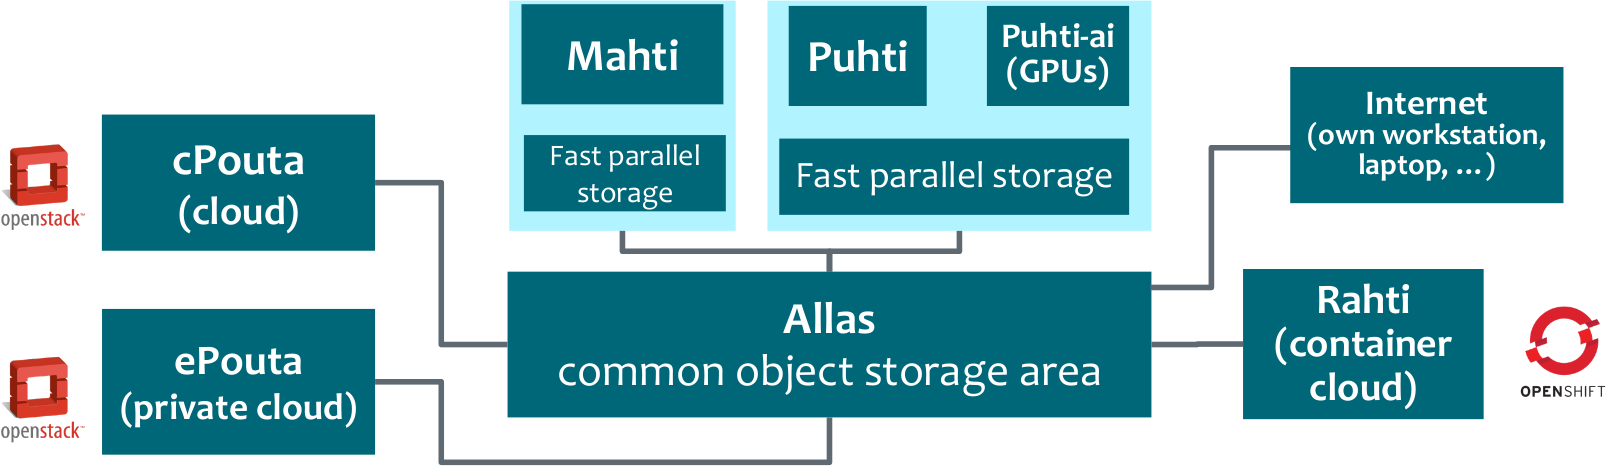
\includegraphics[width=\textwidth]{csc-services}};
    \uncover<2>{\draw[red,ultra thick,rounded corners] (6.5,1.95) rectangle ++(3.7,2.25);}
    \uncover<3>{\draw[red,ultra thick,rounded corners] (-0.2,-0.2) rectangle ++(3.6,3.5);}
    \uncover<4>{\draw[red,ultra thick,rounded corners] (10.7,0.3) rectangle ++(3.5,1.55);}
    \uncover<5>{\draw[red,ultra thick,rounded corners] (4.3,0.33) rectangle ++(5.9,1.45);}
    \uncover<6>{\draw[red,ultra thick,rounded corners] (4.35,1.95) rectangle ++(2.2,2.25);}
  \end{tikzpicture}  
\end{frame}

\section{Puhti supercomputer}

\begin{frame}{Puhti supercomputer}
  \begin{columns}
    \begin{column}{0.76\linewidth}
      \begin{minipage}[c][0.8\textheight][s]{\columnwidth}
      \begin{itemize}
        \vitem \emph{Puhti} has a total of 682 CPU nodes, each with 2$\times$20 Intel Xeon 2,1 GHz cores
        \vitem \emph{Puhti-AI} partition has 80 nodes with \mbox{4 GPUs}
        each $\rightarrow$ 320 GPUs in total
        \vitem NVIDIA V100 GPUs (Volta) with 32 GB of memory
        \vitem Fast network: 2 $\times$ 100 Gbps links to each node
        \vitem Each node has a fast 3.6 TB local NVME disk
      \end{itemize}
      \vfill
      \end{minipage}
    \end{column}
    %% 
    \begin{column}{0.24\linewidth}
      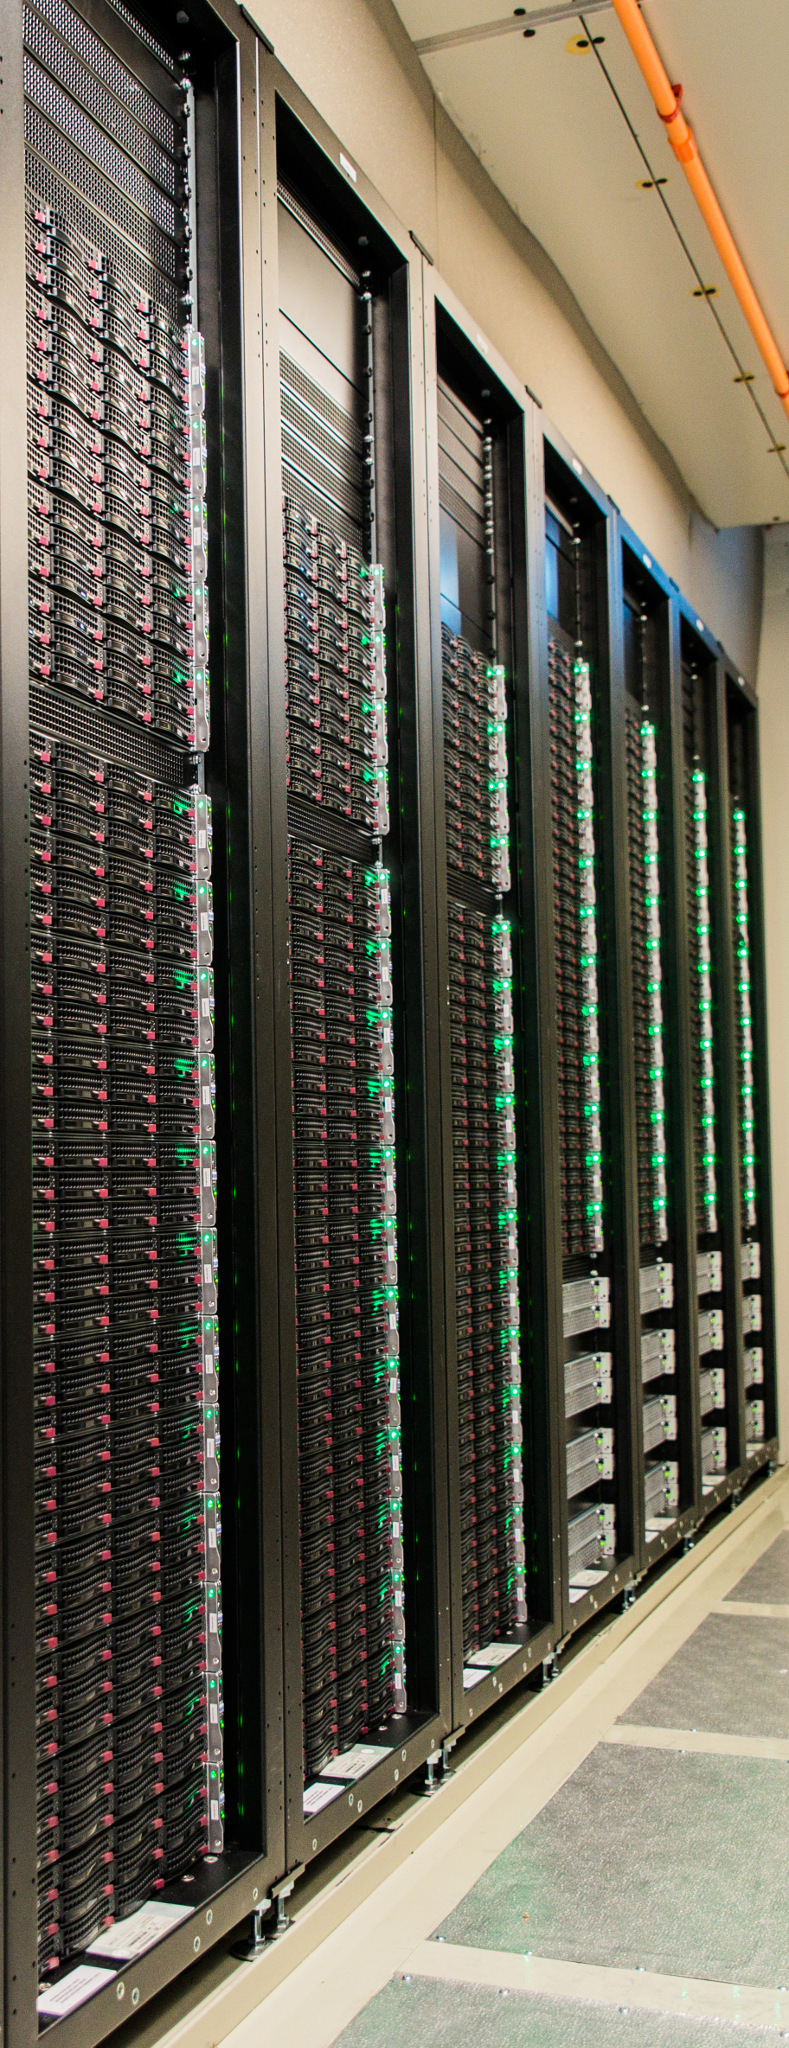
\includegraphics[height=0.8\textheight]{puhti-long}
    \end{column}
  \end{columns}
\end{frame}

\begin{frame}{Getting access to Puhti}
  \link{https://docs.csc.fi/computing/overview/}

  \vspace{1em}

  To use Puhti you need to:
  \begin{itemize}
  \item Have a CSC account
  \item Be member of a CSC project, either by
    \begin{itemize}
    \item creating a new project, or
    \item joining an existing project (ask the PI to add you!)
    \end{itemize}
  \item Finally, the project needs to have Puhti access
  \end{itemize}

  \vspace{1em}

  $\rightarrow$ \quad MyCSC portal: \link{https://my.csc.fi/}

\end{frame}

\begin{frame}[fragile]{Logging in to Puhti}
  \begin{itemize}
  \item Using an ssh client such as OpenSSH or PuTTY
  \item Basic Linux skills are required!
  \item More info: \link{https://docs.csc.fi/computing/connecting/}
  \end{itemize}

  \vspace{1em}

\begin{minted}{shell-session}
$ ssh <csc_username>@puhti.csc.fi
\end{minted}

\begin{minted}{shell-session}
$ ssh <csc_username>@puhti-login2.csc.fi
\end{minted}

\end{frame}

\section{Available software}

\begin{frame}{Supported frameworks}
  We currently support:
  \begin{itemize}
  \item \alert{Python Data} -- collection of Python libraries for data
    analytics and machine learning
  \item \alert{TensorFlow} -- deep learning library for Python
  \item \alert{PyTorch} -- machine learning framework for Python
  \item \alert{MXNet} -- deep learning library for Python
  \item \alert{RAPIDS} -- suite of libraries for data analytics and
    machine learning on GPUs
  \end{itemize}

  {\small \link{https://docs.csc.fi/apps/\#data-analytics-and-machine-learning}}
\end{frame}

\begin{frame}[fragile]{Example: TensorFlow}
  \begin{itemize}
  \vitem First check the application page for instructions:
    \link{https://docs.csc.fi/apps/tensorflow/}
  \vitem Load the default version:
\begin{verbatim}
module load tensorflow
\end{verbatim}
  \vitem or specific version:
\begin{verbatim}
module load tensorflow/2.0.0
\end{verbatim}
  \vitem \alert{Note:} some modules are \emph{Singularity-based}!
\end{itemize}
\vfill
\end{frame}

\begin{frame}[fragile]{What if some package is missing?}
  If you are using our module, but a trivial package is missing \ldots
  \begin{itemize}
  \vitem install it yourself, e.g.,
\begin{verbatim}
pip install --user <packagename>
\end{verbatim}
  \vitem \ldots or if it might be generally useful, send an email to \alert{\tt
      servicedesk@csc.fi} -- we can install it for you!
  \end{itemize}
  \vfill
\end{frame}

\begin{frame}[fragile]{What if some package is missing?}
  \alert{Note:} you can even upgrade an existing package with:
\begin{verbatim}
pip install --user --upgrade <packagename>
\end{verbatim}
  but then you need to adjust the order in which packages are accessed by Python:
{\small
\begin{verbatim}
export PYTHONPATH=~/.local/lib/python3.7/site-packages/:$PYTHONPATH  
\end{verbatim}}
\end{frame}

\begin{frame}[fragile]{What if some package is missing?}
  If you need a specific setup, and our modules are not right for you \ldots
  \begin{itemize}
  \vitem use a virtualenv:
\begin{minted}{shell-session}
$ module purge
$ python3 -m venv myenv
$ source myenv/bin/activate
$ pip install ...
\end{minted}

  \vitem use conda: {\small \link{https://docs.csc.fi/support/tutorials/conda/}}
  \vitem use singularity containers: {\small \link{https://docs.csc.fi/computing/containers/run-existing/}}
    
  \vitem or if generally useful, send an email to \alert{\tt
      servicedesk@csc.fi}
  \end{itemize}
  
\end{frame}

\section{Running jobs on Puhti}

\begin{frame}{Running a job on Puhti}
  \alert{Don't run heavy computing jobs in the login nodes!}
  \vspace{2mm}
  \begin{itemize}
  \item Puhti uses the \emph{Slurm} batch job system
  \item Jobs do not run instantly but are put in a \emph{queue}
  \item Resources (runtime, memory, number of cores) need to be specified
  \end{itemize}

  \vspace{-4mm}
  \begin{center}
    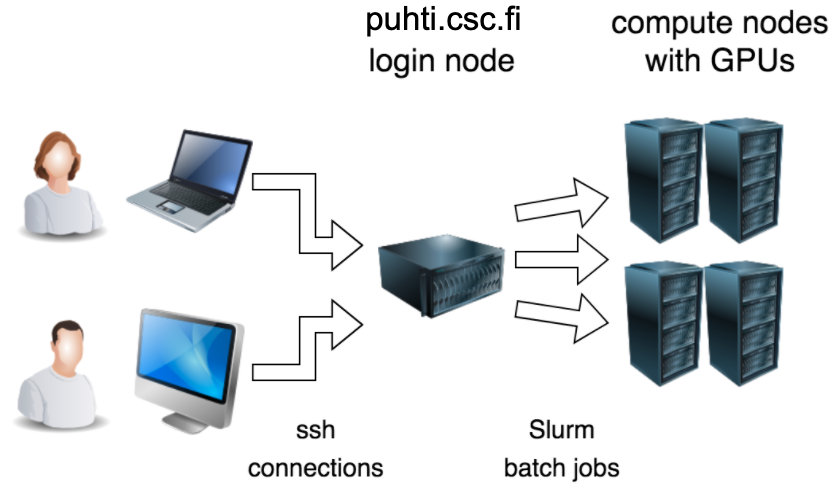
\includegraphics[width=0.55\textwidth]{slurm1.png}    
  \end{center}
\end{frame}

\begin{frame}{Running a job on Puhti}
  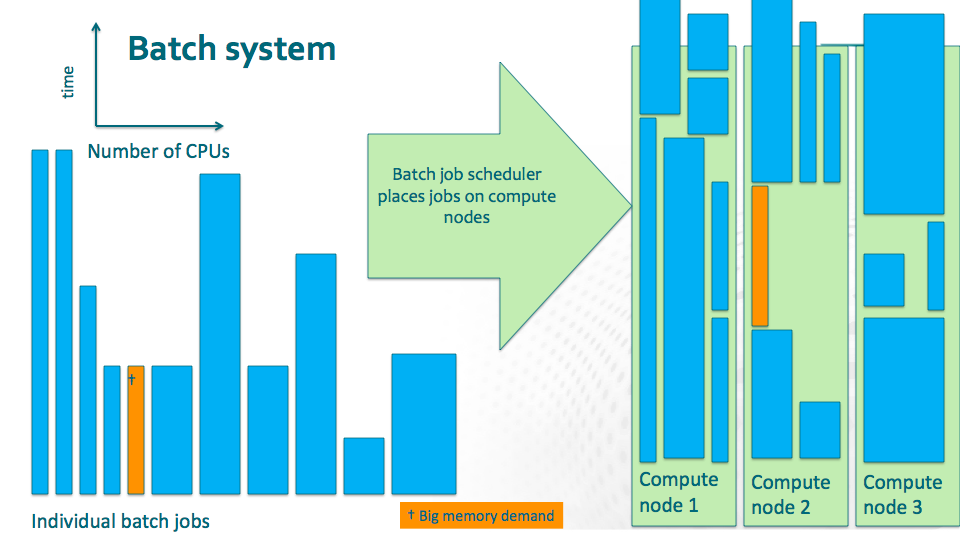
\includegraphics[width=\textwidth]{slurm2.png}
\end{frame}

\begin{frame}[fragile]{Running a job on Puhti}

  Create a job script, for example {\tt run.sh}:
  
\begin{minted}[fontsize=\small,highlightlines={3,8}]{bash}
#!/bin/bash
#SBATCH --account=<project>
#SBATCH --partition=gpu
#SBATCH --ntasks=1
#SBATCH --cpus-per-task=10
#SBATCH --mem=64G
#SBATCH --time=1:00:00
#SBATCH --gres=gpu:v100:1

module load tensorflow/2.0.0
srun python3 myprog.py <options>
\end{minted}

{\small \link{https://docs.csc.fi/computing/running/creating-job-scripts/}}
\end{frame}

\begin{frame}[fragile]{Running a job on Puhti}

  Example job script for Singularity-based modules:
  
\begin{minted}[fontsize=\small,highlightlines={11}]{bash}
#!/bin/bash
#SBATCH --account=<project>
#SBATCH --partition=gpu
#SBATCH --ntasks=1
#SBATCH --cpus-per-task=10
#SBATCH --mem=64G
#SBATCH --time=1:00:00
#SBATCH --gres=gpu:v100:1

module load tensorflow/nvidia-20.03-tf2-py3
srun singularity_wrapper exec python3 myprog.py <options>
\end{minted}

\end{frame}

\begin{frame}[fragile]{Running a job on Puhti}
  Submit the job:
\begin{verbatim}
sbatch run.sh
\end{verbatim}
  \vfill
  
  Check the queue:
\begin{verbatim}
squeue -l -u $USER
\end{verbatim}
  \vfill
  
  Cancel a job:
\begin{verbatim}
scancel <jobid>
\end{verbatim}

  {\small \link{https://docs.csc.fi/computing/running/submitting-jobs/}}
\end{frame}

\section{Data storage}

\begin{frame}{Data storage on Puhti}

  \begin{itemize}
  \item Disk space and \emph{number of files} are limited on Puhti! \\
    {\small $\rightarrow$ We want to ensure that the shared (Lustre) filesystem works
    efficiently for everyone!}
  \item Useful command: {\tt csc-workspaces}
  \end{itemize}

  \vfill

  {\footnotesize
    \begin{tabular}{lllrrl}
             & Owner    & Path                      & Capacity & Number of files & Cleaning \\
    \hline
    home     & Personal & {\tt /users/<user-name>}  & 10 GiB   & 100 000 files   & No \\
    projappl & Project  & {\tt /projappl/<project>} & 50 GiB   & 100 000 files   & No \\
    scratch  & Project  & {\tt /scratch/<project>}  & 1 TiB    & 1 000 000 files & Yes - 90 days \\
    \end{tabular}
  }
  \vfill
  {\small
    Data quotas can be increased via MyCSC!

    \link{https://docs.csc.fi/computing/disk/}}
\end{frame}

\begin{frame}[fragile]{Using Allas}
  \begin{itemize}
  \item store big datasets in Allas, CSC's object storage
  \item download them to project scratch prior to computation
  \item you can also upload trained models (or keep in projappl)
  \end{itemize}

  \vfill
  
  % \begin{verbatim}
\begin{minted}{shell-session}
$ module load allas
$ allas-conf
$ cd /scratch/<your-project>
$ swift download <bucket-name> your-dataset.tar  
\end{minted}
  % \end{verbatim}

  \link{https://docs.csc.fi/data/Allas/}
\end{frame}

\begin{frame}{Large number of files}
  \begin{itemize}
  \vitem Many datasets contain a large number of small files
  \vitem Shared filesystem (Lustre) performs poorly in this scenario \\
    $\rightarrow$ noticable slowdowns for all Puhti users!
  \end{itemize}

  \vfill
  Consider alternatives:

  \begin{itemize}
    \vitem packaging your dataset into larger files                     
    \vitem use NVME fast local storage on GPU nodes
  \end{itemize}

  \vfill
  \emph{More details in webinar part 2!}

\end{frame}

% \begin{frame}{Using more efficient data formats}

%   Instead of many small files, use one or a few bigger files.

%   \vfill
  
%   Examples:

%   \begin{itemize}
%   \vitem TensorFlow's TFRecord format
%   \vitem HDF5
%   \vitem LMDB
%   \vitem ZIP, for example via Python's {\tt zipfile} library
%   \end{itemize}

%   \vfill
% \end{frame}

% \begin{frame}[fragile]{Fast local NVME drive}

%   \begin{itemize}
%   \item All GPU nodes have a local NVME drive
%   \item Just add {\tt nvme:<number-of-GB>} to sbatch {\tt --gres} flag
%   \end{itemize}

% \begin{minted}[fontsize=\footnotesize,highlightlines={8,10,12}]{bash}
% #!/bin/bash
% #SBATCH --account=<project>
% #SBATCH --partition=gpu
% #SBATCH --ntasks=1
% #SBATCH --cpus-per-task=10
% #SBATCH --mem=64G
% #SBATCH --time=1:00:00
% #SBATCH --gres=gpu:v100:1,nvme:100

% tar xf /scratch/<your-project>/your-dataset.tar -C $LOCAL_SCRATCH

% srun python3 myprog.py --data_dir=$LOCAL_SCRATCH <options>
% \end{minted}

% \end{frame}

\section*{Thank you!}

\begin{frame}{Don't forget part 2 of this webinar!}

  \textbf{Machine Learning on Puhti \\
    Part 2: Scaling up and using resources efficiently}

  \begin{itemize}
  \item Efficient data storage
  \item GPU utilization
  \item Multi-GPU and multi-node jobs
  \item Singularity containers
  \end{itemize}

  \vfill

  \begin{tabular}{ll}
    \textbf{Time:}  & Wednesday, June 10, 2020 at 14:00-15:00 \\
    \textbf{Place:} & \link{https://ssl.eventilla.com/event/jJRkz} \\
  \end{tabular}

\end{frame}


\end{document}

%%% Local Variables: 
%%% TeX-command-extra-options: "-shell-escape"
%%% End:
